\section{Descriptive Analysis} \label{isect3}
\subsection{Composition of Household Vulnerability Index}
The study uses household characteristics and other information from
the survey, which are more suitable for calculating the household vulnerability of the surveyed households. Table 4.1 presents various variables used for constructing the households vulnerability index district-wise. Appendix Table 1 presents the VDC-level variables.   

In the year 2006, the Household Vulnerability Index (HVI) ranged from 0.61 to 0.65 across the survey districts. By 2012, minimal changes were observed, with certain VDCs in the study districts experiencing an improvement. For instance, Chainpur VDC in Chitwan improved its vulnerability position from 0.62 in 2006 to 0.61 in 2009 but remained stagnant at 0.61 in 2012. Similarly, Kunjo VDC in Mustang district reduced its vulnerability from 0.65 in 2006 to 0.64 in 2009, but remained stagnant at 0.64 in 2012. Lete VDC in Mustang district exhibited no change in vulnerability from 2006 to 2009 but saw a decrease from 0.63 in 2006 to 0.62 in 2012. Conversely, Hemja VDC in Kaski district maintained the same vulnerability position over the six-year span. The observed phenomenon of households improving little to not improving its positions aligns with the findings of \cite{acharya2008dimension} that households in rural areas face significant vulnerability.\par 
\begin{landscape}
	\begin{table}
		\vspace{-35pt}
		\caption{ Variables used to construct the Vulnerability Index}
		\renewcommand{\arraystretch}{1.15}
		\resizebox{1.7\textwidth}{!}{%
			\begin{tabular}{lccccccccc} \hline
				\textbf{Year}                    & \multicolumn{3}{c}{\textbf{2006}}                                                                                                                                                                    & \multicolumn{3}{c}{\textbf{2009}}                                                                                                                                                                    & \multicolumn{3}{c}{\textbf{2012}}                                                                                                                                                                    \\ \hline
				\textbf{District}                & \textbf{Chitwan}                                                & \textbf{Kaski}                                                  & \textbf{Mustang}                                                 & \textbf{Chitwan}                                                & \textbf{Kaski}                                                  & \textbf{Mustang}                                                 & \textbf{Chitwan}                                                & \textbf{Kaski}                                                  & \textbf{Mustang}                                                 \\ \hline
				\textbf{Human Capital}           &                                                                 &                                                                 &                                                                  &                                                                 &                                                                 &                                                                  &                                                                 &                                                                 &                                                                  \\ 
				hhh\_age                         & \begin{tabular}[c]{@{}c@{}}50.36 \\ (14.15)\end{tabular}        & \begin{tabular}[c]{@{}c@{}}50.14 \\ (14.57)\end{tabular}        & \begin{tabular}[c]{@{}c@{}}52.89  \\ (13.52)\end{tabular}        & \begin{tabular}[c]{@{}c@{}}52.13  \\ (13.75)\end{tabular}       & \begin{tabular}[c]{@{}c@{}}52.00  \\ (13.39)\end{tabular}       & \begin{tabular}[c]{@{}c@{}}54.12  \\ (13.78)\end{tabular}        & \begin{tabular}[c]{@{}c@{}}52.24  \\ (17.20)\end{tabular}       & \begin{tabular}[c]{@{}c@{}}53.52  \\ (13.71)\end{tabular}       & \begin{tabular}[c]{@{}c@{}}55.24  \\ (14.17)\end{tabular}        \\
				hhh\_edu                         & \begin{tabular}[c]{@{}c@{}}3.08  \\ (4.06)\end{tabular}         & \begin{tabular}[c]{@{}c@{}}6.29  \\ (4.97)\end{tabular}         & \begin{tabular}[c]{@{}c@{}}3.05  \\ (3.98)\end{tabular}          & \begin{tabular}[c]{@{}c@{}}2.93  \\ (4.06)\end{tabular}         & \begin{tabular}[c]{@{}c@{}}6.07  \\ (5.23)\end{tabular}         & \begin{tabular}[c]{@{}c@{}}2.94  \\ (3.78)\end{tabular}          & \begin{tabular}[c]{@{}c@{}}2.91  \\ (4.33)\end{tabular}         & \begin{tabular}[c]{@{}c@{}}6.91  \\ (5.07)\end{tabular}         & \begin{tabular}[c]{@{}c@{}}2.90  \\ (4.08)\end{tabular}          \\
				max\_hh\_edu                     & \begin{tabular}[c]{@{}c@{}}8.44  \\ (3.91)\end{tabular}         & \begin{tabular}[c]{@{}c@{}}10.76  \\ (2.90)\end{tabular}        & \begin{tabular}[c]{@{}c@{}}7.64  \\ (3.32)\end{tabular}          & \begin{tabular}[c]{@{}c@{}}9.70  \\ (3.63)\end{tabular}         & \begin{tabular}[c]{@{}c@{}}11.18  \\ (3.94)\end{tabular}        & \begin{tabular}[c]{@{}c@{}}8.04  \\ (3.93)\end{tabular}          & \begin{tabular}[c]{@{}c@{}}9.89  \\ (4.44)\end{tabular}         & \begin{tabular}[c]{@{}c@{}}11.91 \\  (4.03)\end{tabular}        & \begin{tabular}[c]{@{}c@{}}8.22  \\ (3.87)\end{tabular}          \\
				\textbf{Physical Capital}        &                                                                 &                                                                 &                                                                  &                                                                 &                                                                 &                                                                  &                                                                 &                                                                 &                                                                  \\
				implements                       & \begin{tabular}[c]{@{}c@{}}4660.32  \\ (11275.51)\end{tabular}  & \begin{tabular}[c]{@{}c@{}}14057.03  \\ (16860.40)\end{tabular} & \begin{tabular}[c]{@{}c@{}}10360.32  \\ (19629.35)\end{tabular}  & \begin{tabular}[c]{@{}c@{}}10153.80  \\ (23970.96)\end{tabular} & \begin{tabular}[c]{@{}c@{}}30700.04  \\ (46128.42)\end{tabular} & \begin{tabular}[c]{@{}c@{}}15135.16  \\ (25508.99)\end{tabular}  & \begin{tabular}[c]{@{}c@{}}22165.29  \\ (38089.26)\end{tabular} & \begin{tabular}[c]{@{}c@{}}48959.03  \\ (70582.61)\end{tabular} & \begin{tabular}[c]{@{}c@{}}21466.58  \\ (27566.06)\end{tabular}  \\
				livestock                        & \begin{tabular}[c]{@{}c@{}}18532.68  \\ (15428.31)\end{tabular} & \begin{tabular}[c]{@{}c@{}}26573.08  \\ (20411.58)\end{tabular} & \begin{tabular}[c]{@{}c@{}}80387.77  \\ (224589.10)\end{tabular} & \begin{tabular}[c]{@{}c@{}}43936.83  \\ (39679.86)\end{tabular} & \begin{tabular}[c]{@{}c@{}}35690.11  \\ (35760.04)\end{tabular} & \begin{tabular}[c]{@{}c@{}}56165.26  \\ (178639.73)\end{tabular} & \begin{tabular}[c]{@{}c@{}}38993.71  \\ (34330.39)\end{tabular} & \begin{tabular}[c]{@{}c@{}}34635.85  \\ (39306.64)\end{tabular} & \begin{tabular}[c]{@{}c@{}}34114.52  \\ (39335.73)\end{tabular}  \\
				land                             & \begin{tabular}[c]{@{}c@{}}2027.47  \\ (6367.27)\end{tabular}   & \begin{tabular}[c]{@{}c@{}}1187.00  \\ (1013.02)\end{tabular}   & \begin{tabular}[c]{@{}c@{}}2940.39  \\ (2789.36)\end{tabular}    & \begin{tabular}[c]{@{}c@{}}915.91  \\ (765.38)\end{tabular}     & \begin{tabular}[c]{@{}c@{}}1491.41  \\ (2060.26)\end{tabular}   & \begin{tabular}[c]{@{}c@{}}2235.09  \\ (3738.40)\end{tabular}    & \begin{tabular}[c]{@{}c@{}}1041.46  \\ (1136.88)\end{tabular}   & \begin{tabular}[c]{@{}c@{}}1374.96  \\ (2253.95)\end{tabular}   & \begin{tabular}[c]{@{}c@{}}1921.22  \\ (1892.77)\end{tabular}    \\
				\textbf{Social Capital}          &                                                                 &                                                                 &                                                                  &                                                                 &                                                                 &                                                                  &                                                                 &                                                                 &                                                                  \\
				hh\_caste                        & \begin{tabular}[c]{@{}c@{}}0.58  \\ (0.50)\end{tabular}         & \begin{tabular}[c]{@{}c@{}}0.89  \\ (0.32)\end{tabular}         & \begin{tabular}[c]{@{}c@{}}0.49  \\ (0.50)\end{tabular}          & \begin{tabular}[c]{@{}c@{}}0.66  \\ (0.48)\end{tabular}         & \begin{tabular}[c]{@{}c@{}}0.98  \\ (0.14)\end{tabular}         & \begin{tabular}[c]{@{}c@{}}0.58  \\ (0.50)\end{tabular}          & \begin{tabular}[c]{@{}c@{}}0.50  \\ (0.50)\end{tabular}         & \begin{tabular}[c]{@{}c@{}}0.86  \\ (0.50)\end{tabular}         & \begin{tabular}[c]{@{}c@{}}0.59 \\ (0.42)\end{tabular}           \\
				\textbf{Financial Capital}       &                                                                 &                                                                 &                                                                  &                                                                 &                                                                 &                                                                  &                                                                 &                                                                 &                                                                  \\
				bank\_saving                     & \begin{tabular}[c]{@{}c@{}}879.58  \\ (2661.50)\end{tabular}    & \begin{tabular}[c]{@{}c@{}}9663.83  \\ (26812.59)\end{tabular}  & \begin{tabular}[c]{@{}c@{}}31897.65  \\ (79933.66 )\end{tabular} & \begin{tabular}[c]{@{}c@{}}1911.63  \\ (6126.69)\end{tabular}   & \begin{tabular}[c]{@{}c@{}}11937.72  \\ (31025.90)\end{tabular} & \begin{tabular}[c]{@{}c@{}}24536.06  \\ (59338.85)\end{tabular}  & \begin{tabular}[c]{@{}c@{}}11953.55  \\ (31763.88)\end{tabular} & \begin{tabular}[c]{@{}c@{}}25410.64  \\ (66932.36)\end{tabular} & \begin{tabular}[c]{@{}c@{}}48051.24  \\ (104495.00)\end{tabular} \\
				jewellery                        & \begin{tabular}[c]{@{}c@{}}0.00  \\ (0.00)\end{tabular}         & \begin{tabular}[c]{@{}c@{}}0.00  \\ (0.00)\end{tabular}         & \begin{tabular}[c]{@{}c@{}}31662.91  \\ (67846.57)\end{tabular}  & \begin{tabular}[c]{@{}c@{}}4396.88  \\ (6965.54)\end{tabular}   & \begin{tabular}[c]{@{}c@{}}20485.87  \\ (16594.27)\end{tabular} & \begin{tabular}[c]{@{}c@{}}38598.35  \\ (79440.96)\end{tabular}  & \begin{tabular}[c]{@{}c@{}}21477.20  \\ (23620.48)\end{tabular} & \begin{tabular}[c]{@{}c@{}}51605.95  \\ (48463.66)\end{tabular} & \begin{tabular}[c]{@{}c@{}}54132.35  \\ (112328.06)\end{tabular} \\
				\textbf{Livelihood}              &                                                                 &                                                                 &                                                                  &                                                                 &                                                                 &                                                                  &                                                                 &                                                                 &                                                                  \\
				n\_livelihoods                   & \begin{tabular}[c]{@{}c@{}}4.81\\ (0.97)\end{tabular}           & \begin{tabular}[c]{@{}c@{}}4.72\\ (0.91)\end{tabular}           & \begin{tabular}[c]{@{}c@{}}4.56\\ (0.93)\end{tabular}            & \begin{tabular}[c]{@{}c@{}}4.93\\ (1.02)\end{tabular}           & \begin{tabular}[c]{@{}c@{}}4.74\\ (0.91)\end{tabular}           & \begin{tabular}[c]{@{}c@{}}5.11\\ (0.84)\end{tabular}            & \begin{tabular}[c]{@{}c@{}}4.60\\ (0.98)\end{tabular}           & \begin{tabular}[c]{@{}c@{}}4.78\\ (0.90)\end{tabular}           & \begin{tabular}[c]{@{}c@{}}4.60\\ (0.98)\end{tabular}            \\
				\textbf{Household Vulnerability} &                                                                 &                                                                 &                                                                  &                                                                 &                                                                 &                                                                  &                                                                 &                                                                 &                                                                  \\
				HVI                              & \begin{tabular}[c]{@{}c@{}}0.61  \\ (0.05)\end{tabular}         & \begin{tabular}[c]{@{}c@{}}0.62  \\ (0.04)\end{tabular}         & \begin{tabular}[c]{@{}c@{}}0.64  \\ (0.05)\end{tabular}          & \begin{tabular}[c]{@{}c@{}}0.61  \\ (0.05)\end{tabular}         & \begin{tabular}[c]{@{}c@{}}0.62  \\ (0.04)\end{tabular}         & \begin{tabular}[c]{@{}c@{}}0.63  \\ (0.05)\end{tabular}          & \begin{tabular}[c]{@{}c@{}}0.61  \\ (0.05)\end{tabular}         & \begin{tabular}[c]{@{}c@{}}0.62  \\ (0.05)\end{tabular}         & \begin{tabular}[c]{@{}c@{}}0.63  \\ (0.05)\end{tabular}         \\ \hline \hline
			\end{tabular}
		}
		\small{\textit{Note:SD in the parenthesis\\ [-0.9ex]
				Source: Author's Calculation}}
			\label{tab:hvivariables}
	\end{table}
\end{landscape}
	
\subsubsection{Human Capital}	
Household Head Age, Education and Maximum educational attainment by the household member were taken as the Human Capital of the households. Household head age as a measure of experience and knowledge has been taken as a contributing factor in Human Capital of the households. The average age of the household head was 52 years in 2006, 53 in year 2009 and 54 in year 2012 (see table \ref{tab:hvivariables}). This progression in the household head age positively affects human capital.\par 

On household head education, Hemja VDC of Kaski district has made a jump of 6 to 7 mean years of schooling from 2006 to 2012. Similarly, Lete VDC of Mustang district has made a negligible progress of 3.25 to 3.3 mean years of schooling. Chainpur VDC of Chitwan district and Kunjo VDC of Mustang district has made negative progress. This mixed progression of household head educational attainment will have mixed effect on human capital.\par  

All VDCs have made positive improvement in part of maximum educational attainment by the household members. Hemja VDC has the highest mean years of schooling of the household members. It has made a remarkable progress from 10 mean years of schooling to 12 from 2006 to 2012. Chainpur VDC also has followed the similar trajectory. It had mean of 8 years of schooling in 2006 and it improved to 10 by the end of 2012. Lete VDC had 8.14 mean years of schooling in the year 2006 which only slightly improved to 8.7 in the year 2012. Kunjo VDC has the least mean years of educational attainment by the household member with 7.1 years in 2006 to 7.72 in 2012. The improvement in the schooling years would affect the human capital positively.\par 

\subsubsection{Physical Capital}
Chainpur VDC had the least implements in the year 2006 whereas Hemja had the highest level of implements in the same year. But, chainpur made remarkable progress by increasing its implements by 118\%  by the end of 2009 and exactly the same increase by the end of the year 2012. Hemja also experience the same rate of growth of implements in the year 2009 but the rate declined to 59\% in the year 2012. Kunjo and Lete, both VDC of Mustang could improve its implements position in the year 2009 by 77\% and 32\% respectively. However, both VDC had a decline in the growth of the implements in the last wave of the survey. Kunjo's increase of the implements was 69\% and Lete's was only 25\% (see table \ref{tab:hvivariables}).\par  

In part of Livestock holdings, Lete VDC had the highest holding in the year 2006 whereas Chainpur had the least holding of the livestock. However, Chainpur managed to increase its livestock-holding by 137\% at the end of year 2009. But Chainpur VDC's livestock holding declined by 11\% by the end of 2012. Kunjo was the second place after Lete in the livestock holding in year 2006. But, its livestock-holding declined continuously in the following years 2009 and 2012 by 25\% and 11\% respectively. Lete VDC despite holding the most livestock in the year 2006 had a severe decline in its livestock holding placing itself as the least livestock-holding VDC by the end of year 2012. It experienced the decrease of 33\% in the year 2009 and almost 60\% in the year 2012.\par  

Lete VDC had the highest land holding followed by Kunjo VDC in the year 2006. Kaski had the least land holdings in the same year. Chainpur then followed Kaski. In year 2009, Chainpur had a decline of 55\% whereas Kunjo and Lete had a decline of 14\% and 33\% respectively. Hemja, however, increased its land-holding by 26\% by the end of 2009. Chainpur, despite experiencing decrease in land-holding, managed to increase the land-holding by 14\% by the end of 2012. In the same period, all 3 VDCs': Hemja; Kunjo; and Lete experienced decline in the land-holding by 8\%, 13\% and 15\% respectively.\par 

\subsubsection{Social Capital}  
Following \cite{alha2018other, vanneman2006social}, the caste was considered as a social capital. Belonging to the largest caste improves the household's network within the community as well as across the community. Thus it helps the households to negate the effects of uncertain events. So, belonging to largest caste have a negative influence on the household vulnerability. In the year 2006 Hemja had the highest percentage of Household head i.e. 89\% belonging to largest caste. Whereas Kunjo had the least percentage of the household heads belonging to the largest caste in the village. The trend followed with increase in the percentage of the household heads belonging to the largest caste in the year 2009. Chainpur, Hemja, Kunjo and Lete had the percentage change of household heads belonging to largest caste increase by 13\%, 10\%, 19\% and 17\% respectively(see table \ref{tab:hvivariables}).\par  

However, the percentage change declined by 23\% and 48\% for Chainpur and Hemja respectively in the year 2012. Kunjo and Lete, however experience an increase of the percentage of household heads belonging to caste by 65\% and 8\% in the year 2012 respectively.\par 

\subsubsection{Financial Capital}
Bank savings and Jewellery are considered as the financial capitals. The financial capital play a huge part in the welfare of the households.\par 

Lete VDC had the highest bank savings in the year 2006 and the trend continued until the final wave of the survey year 2012. It experienced decline of the saving in the year 2009 relative to 2006 by 11\% but it managed to increase its saving by 114\% by the end of 2012. Chainpur had a opposite experience than that of Lete. It had the least bank saving among all VDCs in the year 2006 and it persisted to have least of it in the final wave of the survey year 2012. However, it managed to increase its own saving by 117\% in the year 2009 and 525\% by the end of 2012.\par 

Kunjo had a fairly fluctuating trend with respect to bank saving. It followed Lete to have the second highest possession of bank saving in the year 2006. Though it managed to maintain the position in terms of ranking it had a decline of 41\% in the second of wave of survey year 2009. In the following wave of the survey it experienced an increase of savings by 54\%. But, it fell below the previous ranking. Hemja had a moderate growth of its saving in the year 2009 of 24\%. The rate leaped to 113\% by the end of 2012 (see table \ref{tab:hvivariables}).\par     

The data for jewellery possession were not available for Chainpur and Hemja VDC for the year 2006. So comparing between Kunjo and Lete, Lete had the highest possession of jewellery. It continued to have the highest jewellery possession in the following wave of surveys. The rate of increase remained moderate of 13\% and 22\% in the year 2009 and 2012 respectively. Kunjo, on the other hand, have aggressively increased its jewellery possession by 45\% in the year 2009 and 80\% in the year 2012.\par 

Data for jewellery possession were available for Chainpur and Hemja for 2009 and 2012. Chainpur had the least possession in the year 2009. But, it managed to increased its possession by 388\% in the year 2012 which is the highest rate of increase among all VDCs. Nonetheless, it persisted in the VDC having the least possession of jewellery in the final wave of survey year 2012.\par

\subsubsection{Livelihood Options}
This includes the diversity of livelihood options that the households in the particular area in the particular period of time. The livelihood is considered a capital because having diversified income can raise household income, reduce risk, and improve their livelihoods \citep{scoones2013livelihoods}. All of the VDCs have a relatively similar livelihood counts. In the year 2006, the number of livelihood strategies that the households adopted ranged from 4.32 to 4.81. Kunjo had the least number of livelihood strategies while Chainpur had a relatively more number of strategies. The average number of livelihood strategies have increased in the year 2009. But, the rate of increase is fairly mild for Chainpur with only 2\% increase and Hemja with only 0.4\%.  As for Kunjo, it had an increase of 11\% in their livelihood counts. Lete had an increase of 12\% in the year 2009. In the year 2012, all VDCs except for Hemja experienced downward sloping livelihood counts. Hemja observed a growth of 0.84\% in livelihood strategies, while Chainpur, Kunjo, and Lete exhibited reduced growth rates of 7\%, 11\%, and 8\%, respectively (see table \ref{tab:hvivariables}).

\begin{figure}[htb!]
	\centering
	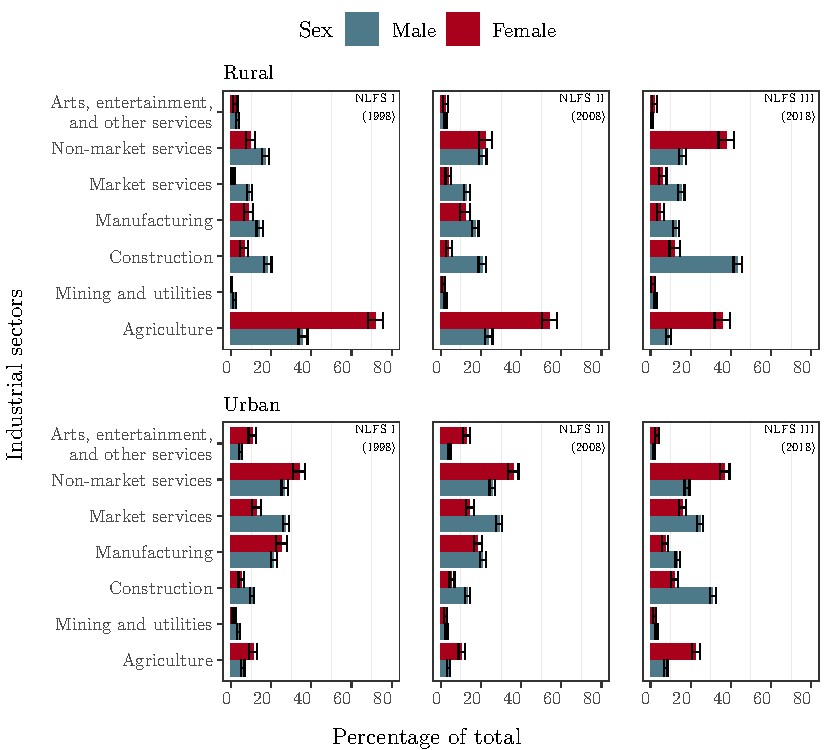
\includegraphics{./figure/industryUrbRur_bar_all_all}
	\caption{Industry-wise employment in rural and urban areas}
	\label{fig:industryUrbRur}
\end{figure}


\begin{figure}[htb!]
	\centering
	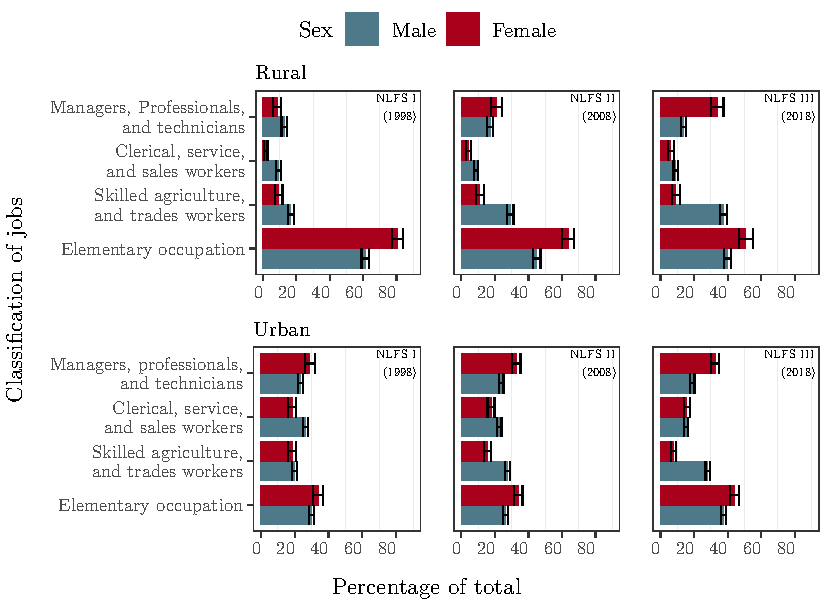
\includegraphics{./figure/occupationUrbRur_bar_all_all}
	\caption{Classification of jobs in rural and urban areas}
	\label{fig:occupationUrbRur}
\end{figure}

After the restoration of democracy in 1990, the country went through a liberalisation and decentralisation of its education sector, with a marked shift in attitude toward education: it was no longer just a social service, but an investment with its own economic returns. This change fostered the growth of the private education sector, particularly in urban areas, catering to families in the burgeoning middle and higher classes~\citep{Carney2009}. The decentralization policies were also well-received -- especially by rural communities, since the policies involved greater community participation in building and operating education institutions, enrolling first-generation graduates all over Nepal. Moreover, during this time, newly available jobs in the service sector that paid more for extra years of schooling created a strong case for higher education, especially among women. Thus, the gender gap in education has progressively narrowed over time (see figure A2 in annex), with both men and women attaining higher levels of education. However, as time has gone on, employed women have outpaced employed men in higher education. This educational phenomenon is not surprising: community colleges have class cohorts with more than two-thirds women, other degree-granting institutions having gender parity~\citep{Ugc2022}.\par 

%\input{tables/laborForceParticipation.tex} 
	
The increase in the number of years of schooling also led the young working-age cohort to stay in education for longer, delaying their entry into the job market. This delay, together with the transition of the economy away from the low-yielding agriculture sector, caused a gradual decline in the labour force participation rate from 50.2\% to 32.4\% over the two decades. By 2018, women’s labour force participation was at 18.2\% from the earlier 31.3\%, whereas men saw even larger decline (from 70.4\% to 50.9\%). Of those who are in the labour force, a complete reversal has occurred in its composition: in 1998, the majority of men and more than two-thirds of women in the labour force were self-employed; by 2018, a majority of men and a larger number of women reported being engaged in wage jobs than self-employment (see table A1 in annex). Overall, between 1998 and 2018, fewer people participated in the labour force, but among those who do, more are in wage-paying jobs than self-employment.\par    

\begin{figure}[htb] 
	\centering
	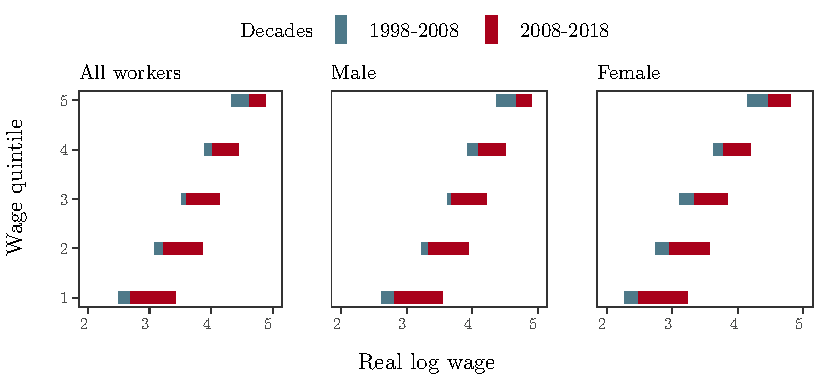
\includegraphics{./figure/log_real_wage_change_NLFS_all}
	\caption{Changes in real wage throughout the wage distribution (1998-2018)}
	\label{fig:wagechangeAll}
\end{figure} 

In the two decades we investigated, wage-earners saw their earnings improve in real terms. The increase in wages in the first decade was negligible: only the highest quintile saw sustained progress which exacerbated the inter-quintile wage spread, especially among men (see table A2 in annex). In terms of gender, women more greatly benefited from the changes in the first decade (see figure \ref{fig:wagechangeAll}). In contrast, between 2008 and 2018, we see substantial wage improvements for both genders across all quintiles. In this decade too, women saw larger gains, and they improved their position relative to men. Women in the highest wage quintile experienced substantial wage improvements and came quite close to the highest-earning men. Consequently, the gender wage gap decreased all around, with the sharpest decline in the highest quintile group. With time, the wage distributions shifted, and the largest improvement came at the lower end of the distribution. This pro-poor shift compressed real wages across both genders, negating the increase in the wage spread of the first decade.\par

Wage evolutions differed substantially between rural and urban areas (see figure A1 in the annex). In the first decade, development in urban areas was anti-poor, with people in the bottom three quintiles seeing either stagnant or eroding real wages. At the same time, rural areas saw improvements across all groups that brought them closer to the urban wages. In the second decade, wages improved across both areas, but larger rural gains narrowed the urban-rural wage divide. A probable cause for this narrowing is the out-migration (mostly of men) that largely occurred in the second decade. This out-migration decreased the rural labour supply, pushing rural wages up toward parity with urban wages. See table \ref{tab:SummarySSVE} for further details on observed characteristics across years.\par 

%On an average, employed males are generally 3 years older than employed females, which is consistent in each survey rounds; see table \ref{tab:SummarySSVE}. But, the average age of employed has increased approximately by 2 years for both genders in the same time. Also, the employed females in 2018, who are overwhelmingly from urban areas, come from families with household heads who are more educated than their male counterparts. In terms of ethnicity, there has been increased employment among Madheshi and Dalit individuals between 1998 and 2008, with further improvement specifically for the Dalit community in 2018. Generally, Khas and Janajati males dominate the job market.\par





